\documentclass[12pt,a4paper]{article}
\usepackage[ngerman]{babel}
\usepackage[utf8]{inputenc}
\usepackage{hyperref}
\usepackage{xcolor}
\usepackage{graphicx}

\title{ORES Preparation}
\author{Tom Gülenman}
\begin{document}
\maketitle
\textit{Disclaimer: No guarantee for the correctness of information / explanations / sources is given.}
\section{Sources}
\subsection{ORES direct sources}
\begin{itemize}
\item ORES: Facilitating re-mediation of Wikipedia’s socio-technical problems. 
(2018)
\item \href{https://blog.wikimedia.org/2015/11/30/artificial-intelligence-x-ray-specs/}{Blogpost} (https://blog.wikimedia.org/2015/11/30/artificial-intelligence-x-ray-specs/)
\item \href{https://www.mediawiki.org/wiki/ORES}{Wikimedia Page} (https://www.mediawiki.org/wiki/ORES)
\item \href{https://www.mediawiki.org/wiki/ORES/FAQ}{ORES FAQ} (https://www.mediawiki.org/wiki/ORES/FAQ)
\end{itemize}
\subsection{Other possibility to use ORES}
\begin{itemize}
\item \href{https://en.wikipedia.org/wiki/User:Fuzheado/ORES_experiment}{ORES Experiment} (https://en.wikipedia.org/wiki/User:Fuzheado/ORES\_experiment)
\end{itemize}
\subsection{Current ORES UI (\(\rightarrow\) work on an improvement here)}
\begin{itemize}
\item \href{https://ores.wikimedia.org/ui/}{ORES GUI} (https://ores.wikimedia.org/ui/)
\end{itemize}
\subsection{Also interesting in that context}
\begin{itemize}
\item \href{https://research.google.com/bigpicture/attacking-discrimination-in-ml/}{Google} (not sure if useful, https://research.google.com/bigpicture/attacking-discrimination-in-ml/)
\end{itemize}
\section{ORES: Facilitating re-mediation of Wikipedia’s socio-technical problems.}
\subsection{Abstract}
\subsubsection{point of departure:}
\begin{itemize}
\item Wikipedia's challenges and community's value change, but algorithmic support systems remain stagnant
\item Conversation about quality of control and what place algorithms have remains exclusive to few experts
\end{itemize}
\subsubsection{proposed solution: ORES...}
\begin{itemize}
\item ... to open up socio-technical conversations
\(\rightarrow\) and enable theoretical mechanisms of social change
\end{itemize}
\subsection{Introduction}
\begin{itemize}
\item As every other major platform, that is based on user-generated content, moderation has been relying on artificial intelligence
\item But Wikipedia's approach is different in terms of \textit{Fairness}, \textit{Accountability}, \textit{Transparency in ML}
\(\leftarrow\) strong ideological principles of openness of the volunteer community
\item \textbf{ORES} pushes innovations in openness in ML even further:
\begin{itemize}
\item volunteers \textit{curate labeled training data} from variety of sources for particular prupose
\item commission production of machine classifier
\item make classifier available via API
\(\rightarrow\) classifying on criteria like ``not / damaging'', ``good/bad faith'', quality scale
\end{itemize}
\end{itemize}
\subsubsection{Audiences for this work}
\begin{itemize}
\item ORES is also the implementation of dominant recommendations for algorithmic system builders around transparency and community consent
\item ``automation in Wikipedia has generally made it more difficult for newcomers''
\item ``ORES is an advanced algorithmic
prediction service for Wikipedians that is designed to democratize the development of work
process support tools to a wider audience'' \(\rightarrow\) not \textbf{directly} solve quality/newcomer problem
\end{itemize}
\subsubsection{Genre: A systems paper and a work study paper}
-
\subsection{Related Work}
\subsubsection{The politics of algorithms}
\begin{itemize}
\item Relevance of algorithms is increasing in social and political life \(\rightarrow\) new questions of fairness and transparency
\item In this paper: Wikipedia's algorithmic quality control and socialization practices
\end{itemize}
\subsubsection{Machine prediction in support of open production}
State-of-the-art:
\begin{itemize}
\item Vandalism detection
\begin{enumerate}
\item Automated bots reverting most obvious vandalism
\item ``vandal fighers'': not fully automated bots for less obvious vandalism
\item Watchlists of experienced Wikipedia editors
\end{enumerate}
\item Task routing: SuggestBot routes attention to important, but low quality articles
\end{itemize}
\subsubsection{The Rise and Decline: Wikipedia's socio-technical problems}
\begin{itemize}
\item Problem context
\begin{itemize}
\item Wikipedia grew exponentially between 2005 and 2007
\item Scaling was a struggle \(\rightarrow\) efficiency of quality and damage control \(>\) positive experience of newcomers
\item Prioritizing efficiency by using ML \(\rightarrow\) decline of good-faith newcomers and overall editors
\end{itemize}
\item Countermeasures
\begin{itemize}
\item multiple initiatives, e.g. ``The Teahouse'', a newcomer help space (meet exp. users)
\end{itemize}
\item Results
\begin{itemize}
\item The dominant quality control systems remained unchanged
\item Most efforts did not show any gains in newcomer retention
\item Experiments have been done with control that highlights good editors who run into trouble
\end{itemize}
\end{itemize}
\subsection{Design rationale}
Wikipedia's problems are systemic (necessity for ML with its conseq.) but with no apparent system-level solutions.

How does Wikipedia function (processes, policies etc.)? \(\rightarrow\) How to use ML to adress problems?

\subsubsection{The context: Wikipedia as a genre ecology}
\begin{itemize}
\item Processes not centrally planned
\item ``Bots and human-computation tools mediate the meaning of
policies and how Wikipedia enacts quality management''
\end{itemize}
\subsubsection{The problem: Wikipedia's problems with automated mediation}
Again: trading human newcomer socialization for efficient quality control \(\rightarrow\) decline in retention of new editors.

Genre ecology here \(=^?\) mediation of policy and the design of software
\subsubsection{The complication: Making change in an decentralized ecology}
\begin{itemize}
\item General interest in balancing quality/efficiency and
diversity/welcomingness more effectively exists
\item Where are the designers able to make such a change?
\end{itemize}
\subsubsection{The goal: Expanding the margins of the ecology}
\begin{itemize}
\item The barrier: needing to know about ML classification models for quality control
\item Two options to lower the barrier to create quality control: 
\begin{enumerate}
\item increase general literacy around ML
\item minimize need to deeply understand ML \(\leftarrow\) ORES
\end{enumerate}
\item How does ORES do that?
\begin{itemize}
\item Support multiple classifiers at scale
\item Design accessible interfaces to engage with those classifiers
\item engage in basic outreach efforts
\end{itemize}
\end{itemize}
\subsection{The ORES System}
Architectural overview
\subsubsection{Conceptual architecture}
Components:
\begin{itemize}
\item Collection of machine classifier models (using varied sources of training data)
\begin{itemize}
\item For Wikipedia: models related to damage-detection, quality assessment and topic-routing
\item But adaptable to wide range of other models
\end{itemize}
\end{itemize}
Making models available:
\begin{itemize}
\item ``Container service''
\item Containers = Models referred to as \textit{ScoringModel}s
\item \textit{ScoringModel}s contain metadata:
\begin{itemize}
\item When model was trained/tested
\item Which features are necessary for making prediction
\item Predictions are JSON documents
\end{itemize}
\item Access \textit{ScoringModel}s via RESTful HTTP interface and show users JSON documents = predictions
\end{itemize}
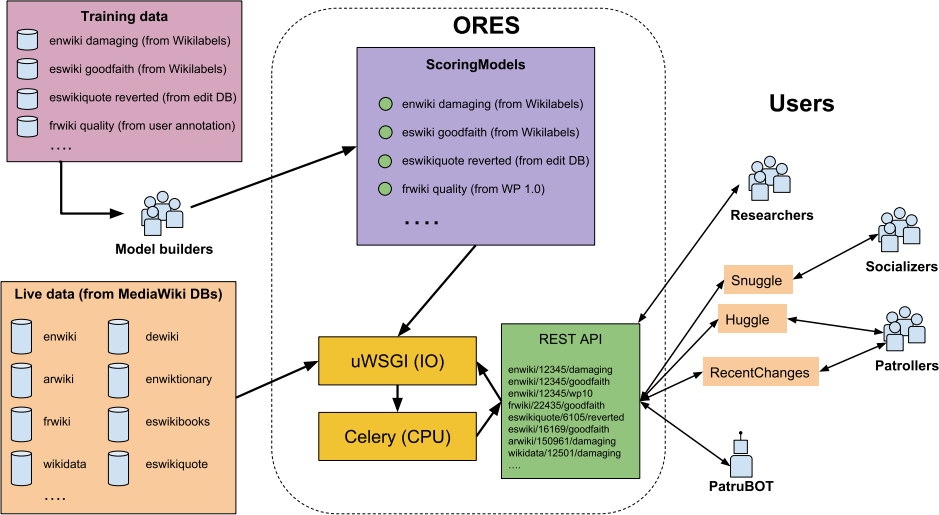
\includegraphics[scale=0.4]{ORESML}
\subsubsection{Scaling \& robustness}
ORES uses distributed computation:
\begin{itemize}
\item IO workers (\textbf{uwsgi}) \(\leftarrow\) requests are split between those, necess. data is gathered using external APIs
\item Computation workers (\textbf{celery}) \(\leftarrow\) data is then split into job queue 
\end{itemize}
\begin{description}
\item \(\Rightarrow\) Efficient use of resources and scalable: IO and CPU workers can be added in multiple datacenters if needed
\item \(\Rightarrow\) Robust (fault tolerant): servers can fail without failing the whole service
\end{description}
\subsubsection{Real-time processing}
ORES's most common use case: real-time processing of edits, e.g. counter-vandalism withing seconds of when edits are made (tools like Huggle)
\begin{itemize}
\item Single score. ORES generates score from scratch if requested in real-time. 1.1 - 1.9 seconds.
\item Caching and precaching. Scores of edits that have been recently generated: 20X faster (50ms)
\end{itemize}
\subsubsection{Batch processing}
\begin{itemize}
\item Wikipedia's bots rely on batch processing \(\rightarrow\) ORES needs to support \textbf{sudden, high-intensity querying}
\item Splitting IO (gather data) and CPU operations into distinct stages \(\rightarrow\) 5X increase in time for large requests
\item Worst case: 1 million revisions in < 24 hours
\end{itemize}
\subsubsection{Empirical access patterns}
\begin{itemize}
\item ORES supports 78 different models and 37 different language-specific wikis
\item Generally 50-125 requests per minute from tools that use ORES predictions
\item Sometimes up to 400-500 /min
\item Precaching requests: (from graphic) 600-800 /min up to 1.1k /min
\end{itemize}
\subsection{Innovations in Openness}
\begin{itemize}
\item Keep the system open for review, critique, iteration
\item System = flow of data from random samples through model training and evaluation
\(\Rightarrow\) enable flexibility in the use of ORES
\end{itemize}


\subsubsection{Collaboratively labeled data}
Two ways of gathering labeled data for ORES' models:
\begin{enumerate}
\item Found traces
\begin{itemize}
\item Taking sample of edits and labeling them as \textit{reverted\_for\_damage} if reverted within 48 hours, reverting editor \(\neq\) author, edit not restored
\item Only make use of this when manually labeled data is not available (because  \textit{reverted\_for\_damage} is problematic: no information about good/bad faith, content dispute etc)
\item Other case of found traces: Article quality assessment (``\textit{wp10}'')
\end{itemize}
\item Manual labeling
\begin{itemize}
\item Asking Wikipedians judgements on examples from their wikis
\item High up-front expense of human labor but \(\Rightarrow\) models that give predictions that make sense to these communities
\item Wikipedians are also asked to distinguish btw. \textit{damaging}/\textit{good} and \textit{good faith}/\textit{vandalism}
\item Result: two different models \(\rightarrow\) Users can search for good-faith mistakes, vandalism or all damaging edits
\end{itemize}
\end{enumerate}
\subsubsection{Threshold optimization}
\begin{itemize}
\item Operational concerns (examples):
\begin{itemize}
\item Catch ``all'' vandalism before it is allowed to stick in Wikipedia for long (\(\rightarrow\) concern around \textbf{recall} of a damage prediction model) (recall: catching damaging edits)
\item Review as few edits as possible (\(\rightarrow\) concern about filter rate)
\end{itemize}
\begin{description}
\item Important: find threshold of prediction likelihood that optimizes filter-rate at high level of recall.
\item \(\Rightarrow\) Find best trade-off btw efficiency and reliability of filter
\item = \textbf{threshold optimizations}
\begin{itemize}
\item Filter-rate: workload of vandal-fighters is reduced by 88\% 
\item Recall: Catching 75\% of (the most) damaging edits
\item Likelihood: 0.299
\item Precision: 0.215 \(\rightarrow\)  ``How often is it that when an edit is predicted to be “damaging” it actually is?''
\end{itemize}
\end{description}
\end{itemize}
\subsubsection{Dependency injection and interrogability}
ORES is designed to host machine classifiers but is suited to other scoring paradigms as well.
\begin{itemize}
\item Dependency injection
\begin{itemize}
\item Serve multiple scores in same request: e.g. ``edit type'', ``damaging'' etc. scores;
\item These models depend on features related to edit \textit{diff}
\item ORES combines features required for models and extracts them with their shared dependencies together
\begin{description}
\item \(\Rightarrow\) \textbf{Efficiency} of multiple requests is roughly the same as for one req
\end{description}
\end{itemize}
\item Flexibility
\begin{itemize}
\item Interrogability: exposing how ORES makes predictions; inject own features as user, e.g. what if this same edit was made by an unknown user (Fig.4 ``damaging'' false 0.938 \% \(\rightarrow\) 0.912\%)
\item ORES is in that way also used to suggest work to new editors (by asking what change one more image / header / citation etc make)
\end{itemize}
\end{itemize}
\subsection{Adoption Patterns}
ORES: make edit quality predictions available \(\rightarrow\) lower barrier to experimentation
\subsubsection{Showcase tools}
\begin{enumerate}
\item \textbf{ScoredRevisions}
\begin{itemize}
\item Javascript-based gadget
\item Submits requests to ORES to score edits
\item Then highlights Edits as \colorbox{red}{``damaging''}, \colorbox{yellow}{worth reviewing} or not at all in color.
\item Limits: requesting 50-500 edits at once (all the edits on a page!) \(\rightarrow\) 30s-2m; not possible to filter edits to only show damaging f.ex.
\end{itemize}
\item \textbf{The ORES Review Tool}
\begin{itemize}
\item MediaWiki extension in PHP
\item Offline process scoring all recent edits to Wikipedia; storing them in a table for querying and quick access
\item Similar to \textbf{ScoredRevisions}, but pre-caching scores \(\rightarrow\) rendering highlights as the page loaded and enabling filtering
\item Successful: around 26k/70k editors manually enabled this feature (April 2017)
\end{itemize}
\end{enumerate}
\subsubsection{Adoption in current tools}
Many developers quickly adopted ORES in their tools for counter-vandalism, but also article-quality. E.g. SuggestBot included ORES predictions in their tables of recommendations.
\subsubsection{Development of new tools}
New tools have been dev. since ORES' release that may not have been dev at all otherwise
\begin{itemize}
\item e.g. Redesign of MediaWiki's Special:RecentChanges interface \(\rightarrow\) conclusion of the ORES Review Tool.
\item Before ORES Wikipedia was (maybe) the only wiki to use ML to revert vandalism. Sincec ORES release that has changed: e.g. PatruBOT in Spanish Wikipedia
\item Wiki Education Foundation: supporting classroom activities that involve editing Wikipedia
\end{itemize}
\subsection{Case studies in reflection}
With the first deployment of ORES came also lots of \textbf{false-positives} reports from users.
\subsubsection{Report mistakes (Wikidata)}
\begin{itemize}
\item The deployement of the first models for Wikidata was accompanied deployment of the ``Report mistakes''-site for users to report \textbf{false-positives}
\item ORES devs learned in what ways Wikidata editor's understandings differed from the feature extraction process
\item The resulting improvements were made public in form of a table
\end{itemize}
\subsubsection{Patrolling/ORES (Italian Wikipedia)}
\begin{itemize}
\item Similar way: report sites (with categories)
\item Example: ``ha'' (Italian \textit{have})
\end{itemize}
\subsubsection{PatruBOT (Spanish Wikipedia)}
\begin{itemize}
\item Another bot reverting edits using ORES prediction
\item Not working very well though, currently disabled
\end{itemize}
\subsubsection{Bias against anonymous editors}
\begin{itemize}
\item Context:
\begin{itemize}
\item At the time using Linear SVM (*) estimators to build classifiers
\item Considering transition towards ensemble stategies like GradientBoosting (*) and RandomForest estimators
\end{itemize}
\item Started rec. reports that ORES dmg detection was biased against anonym. editors
\item Used injection feature to look at how the prediction models changed if the same edit was made by diff. editor
\item Injection analysis confirmed that point (Fig. 7 p.22)
\item Improvements were made to the modeling strategy to mitigate the problem
\(\Rightarrow\) Feedback proved very valuable
\end{itemize}
\subsubsection{Discussion}
\begin{itemize}
\item Understandings and models were refined with the help of feedback from the communities
\item Spanish Wikipedians are still discussing what false discovery rate would be acceptable, or if any revert is acceptable without human intervention
\end{itemize}
\subsection{Conclusion and Future Work}
\begin{itemize}
\item ORES was created by a community that has only a fraction of the resources that for-profit organizations as Facebook and Google have
\item The deployed technology will not be a black box to users, but offers classifiers to be open to skeptical reinterpretation
\item ORES: socio-technical, CSCW approach to fairness, accountability and transparency in ML
\end{itemize}
\subsubsection{``Hearing to speech'': lowering barriers to participation}
\begin{itemize}
\item Goal
\begin{itemize}
\item not ``\textbf{speaking to be heard}'' (build exact technology \textit{we} think is right for Wikipedia)
\item but ``\textbf{hearing to speech}''
\(\Rightarrow\) ``What is preventing others from getting involved in this ocnversation?'' and lower those barriers
\end{itemize}
\item Values that ORES should help sustain: more complete balance of efficient quality control and newcomer support
\item ORES targets early precursors of social change: ecological health and critical reflection
\end{itemize}
\subsubsection{Ecological health}
\begin{itemize}
\item The technological conversation around quality control represents a substantial shift from post-edit boundary to pre-review training for newcomers
\end{itemize}
\subsubsection{Critical reflection}
\begin{itemize}
\item Both case studies show that reflection over algorithms in quality control is taking place
\item Surprising alternatve uses of ORES have surfaced
\item Much concern from Wikipedians has surfaced about a direction of change for quality control
\item Wikipedians collaborate to build information about trends in ORES' mistakes
\end{itemize}
\subsubsection{Future work}
\begin{itemize}
\item Imporved crowd-baseed auditing tools
\(\rightarrow\) Future devs: impl. structured means to discuss the predictions of machine models (e.g. report \textit{false positives})
\item Make it easier to query a ORES mistakes DB \(\rightarrow\) users can show that biases and the resulting problems exist and coordinate with each other and even turn the model / ORES off
\item ``we also see potential in allowing Wikipedians, the denizens of Wikipedia, to freely
train, test, and use their own prediction models without our engineering team involved in
the process'' (p. 26)
\item Currently only someone with strong modeling and programming background can deploy models
\end{itemize}

\section{\href{https://blog.wikimedia.org/2015/11/30/artificial-intelligence-x-ray-specs/}{Blogpost}: Artificial intelligence service ``ORES'' gives Wikipedians X-ray specs to see through bad edits (November 30th, 2015)}
\begin{itemize}
\item New artificial intelligence to help discover damaging edits and ``score'' the quality of any Wikipedia article
\item ...as an open Web service
\item Hope: ORES will enable advancements in how we do quality control
\end{itemize}
\subsection{How it works}
\begin{itemize}
\item Automated edit and article quality classification to everyone via APIs
\item https://ores.wmflabs.org/scores/\colorbox{gray}{enwiki}/\colorbox{pink}{damaging}/\colorbox{green}{620376896}
\begin{itemize}
\item \colorbox{gray}{Type of Wiki} (English Wikipedia)
\item \colorbox{pink}{Model}
\item \colorbox{green}{Revision ID} (found at the top of a page)
\end{itemize}
\(\Rightarrow\) API returns results in JSON
\item Revision scores can be used in ``your'' application by calling an available ORES endpoint (\(\rightarrow\) this link is not available anymore)
\end{itemize}
\subsection{Towards better quality control}
\begin{itemize}
\item There have been automated tools (Huggle, STiki) and bots (ClueBot NG) to help with damage detection before
\item Problem with those: newcomer barriers such as encouraging rejection of new editors' changed (as if made in \textit{bad faith})
\item ORES: newcomer support and training spaces (like \textit{Teahouse} and \textit{Help desk})
\begin{description}
\item \(\Rightarrow\) \textbf{ORES decouples damage prediction from quality control}
\item \(\Rightarrow\) New tools and processes that are efficient and welcoming to new editors
\end{description}
\end{itemize}
\subsection{A feminist inspiration}
\begin{itemize}
\item ``Please exercise extreme caution to avoid ecnoding racism or other biases into an AI scheme.''
\begin{description}
\item Recent research has called attention to increased technological influence on governance and power dynamics
\item SW dvpmt in collab. envrmt req. application of many diff. perspectives
\item \(\Rightarrow\) ``hearing to speech'' strategy
\end{description}
\end{itemize}
\subsection{Who's using revision scores}
Examples:
\begin{itemize}
\item Vandalism fighters like Huggle
\item Snuggle uses edit quality scores to direct good-faith newcomeres to appropriate mentoring spaces
\item Wiki Education Foundation: surfaces most valuable contributions made by students in an education program
\end{itemize}
\subsection{What's next}
\begin{itemize}
\item Supporting more wikis
\item Edit type classification: categorize edits by the type of work performed (\(\rightarrow\) edit type model)
\item Bias detection: collecting feedback on mistakes and devping strat.s for detecting bias in the models
\end{itemize}

\section{\href{https://www.mediawiki.org/wiki/ORES}{Wikimedia Page}: ORES}
\begin{description}
\item Only new information from now on...
\end{description}
\begin{itemize}
\item Two levels of support for edit quality prediction models:
\begin{itemize}
\item Basic support: Build model on history of edits (bad edits have been reverted, good ones haven't); problem: reverts too many edits (\colorbox{cyan}{reverted})
\item Advanced support: Ask editors to train ORES which edits are damaging and which are in \textit{goodfaith} (\colorbox{cyan}{damaging}) (\colorbox{cyan}{goodfaith})
\end{itemize}
\item Curation support: Also predict if new articles will be deleted (\colorbox{cyan}{draftquality})
\item Assessment scale support
\begin{itemize}
\item Large Wikipedias periodically evaluate quality of articles
\item Quality scale: FA, FL, A, GA, B, C, Start, Stub, List, Assessed, Unassessed
\begin{description}
\item \(\Rightarrow\) Helps gauge the progress and identify popular articles that are low quality f.ex.
\item \(\Rightarrow\) Article quality model (\colorbox{cyan}{articlequality})
\end{description}
\item Article quality measured by (examples):
\begin{itemize}
\item Number of section
\item Infobox?
\item Number of references
\item Ref.s using ``cite'' template?
\begin{description}
\item \(\Rightarrow\) Not evaluating the quality of writing, \textbf{but} these measured structural characteristics seem to correlate strongly with good writing \(\rightarrow\) models work well in practice
\end{description}
\end{itemize}
\end{itemize}
\item See page for more info on \textbf{How to use ORES}
\end{itemize}
\section{\href{https://www.mediawiki.org/wiki/ORES/FAQ}{ORES FAQ}}
\begin{itemize}
\item ORES scores: allow humans and machine to work together
\begin{description}
\item e.g. \textbf{patrollers}: human users who help determine whether edits are dmging
\end{description}
\item How to use ORES: 
\begin{itemize}
\item Built-in: RecentChanges, Watchlist and Contributions pages for supported wikis
\begin{description}
\item \(\rightarrow\) See \href{https://en.wikipedia.org/wiki/Special:RecentChanges?hidebots=1&hidecategorization=1&hideWikibase=1&limit=50&days=7&urlversion=2}{Recent changes with filter interface}
\end{description}
\item ``My'' editing activities: find a tool that uses ORES or directly via API (\url{https://ores.wikimedia.org/v3/scores/enwiki/234234320/damaging})
\item What tools are avail. to use ORES? (\url{https://www.mediawiki.org/wiki/ORES/Applications})
\begin{description}
\item Categories:
\end{description}
\begin{itemize}
\item Integration with MediaWiki: RecentChanges, Watchlist
\item Counter-vandalism
\item New page patrolling
\item Article quality assessment
\item Task routing
\end{itemize}
\end{itemize}
\end{itemize}

\section{\href{https://en.wikipedia.org/wiki/User:Fuzheado/ORES_experiment}{ORES Experiment}}
\textit{Experimenting with Revscore and ORES in the Classroom}
\begin{itemize}
\item Teaching students how to edit Wikipedia
\begin{itemize}
\item Before ORES: Hoping the changes stick around
\item With ORES: Getting immediate feedback (stub, start, C ...) and going back for more editing
\end{itemize}
\item Experiment: 13 students (+ 1 teacher) to improve articles in 1 hour and check results with ORES
\begin{itemize}
\item 8/14 articles classified as \textbf{Start}, others as \textbf{Stub}
\item Results: 9/14 jumped up 1 ranking, 1/14 jumped up 2 rankings
\end{itemize}
\item Conclusion (more or less in the article): Gamification elements in form of scores and instant feedback but also through 1 hour challenge
\begin{description}
\item \(\Rightarrow\) Seems like an excellent method to raise motivation!
\end{description}
\end{itemize}
\section{Current \href{https://ores.wikimedia.org/ui/}{ORES GUI}}
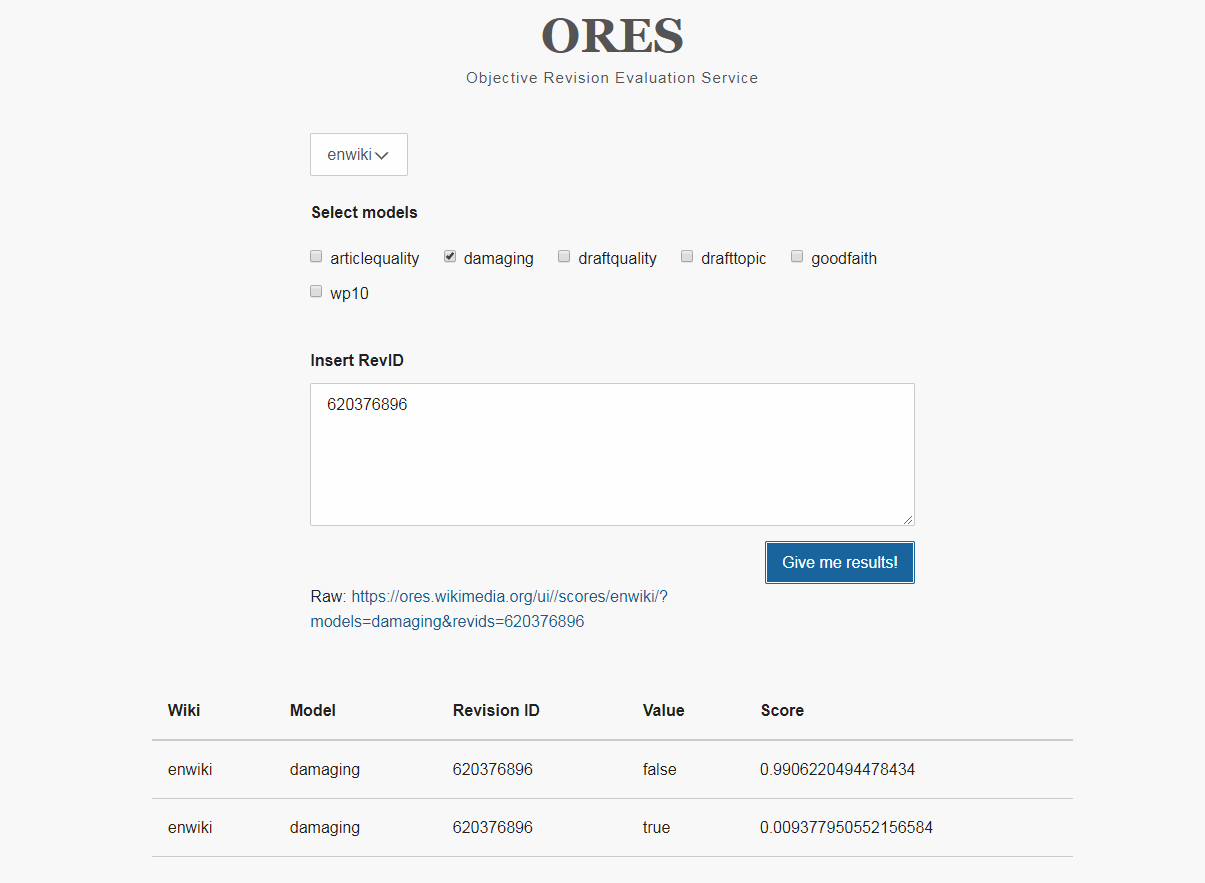
\includegraphics[scale=0.35]{ORESGUI.png}

\section{Google: \href{https://research.google.com/bigpicture/attacking-discrimination-in-ml/}{Attacking discrimination in machine learning}}
\subsection{Attacking discrimination with smarter machine learning}
\begin{itemize}
\item Threshold classifier: make yes/no decision, putting things in one category or another
\begin{description}
\item \(\Rightarrow\) Look at how they work, ways they can be unfair and how to make them fair again
\item \(\Rightarrow\) Example here: loan granting scenario
\end{description}
\item Credit scores: representing the probability of payback
\begin{description}
\item \(\Rightarrow\) One number calculated from numerous factors
\end{description}
\item Bank then picks a \textbf{threshold} and people with credit scores below that are denied the loan
\end{itemize}
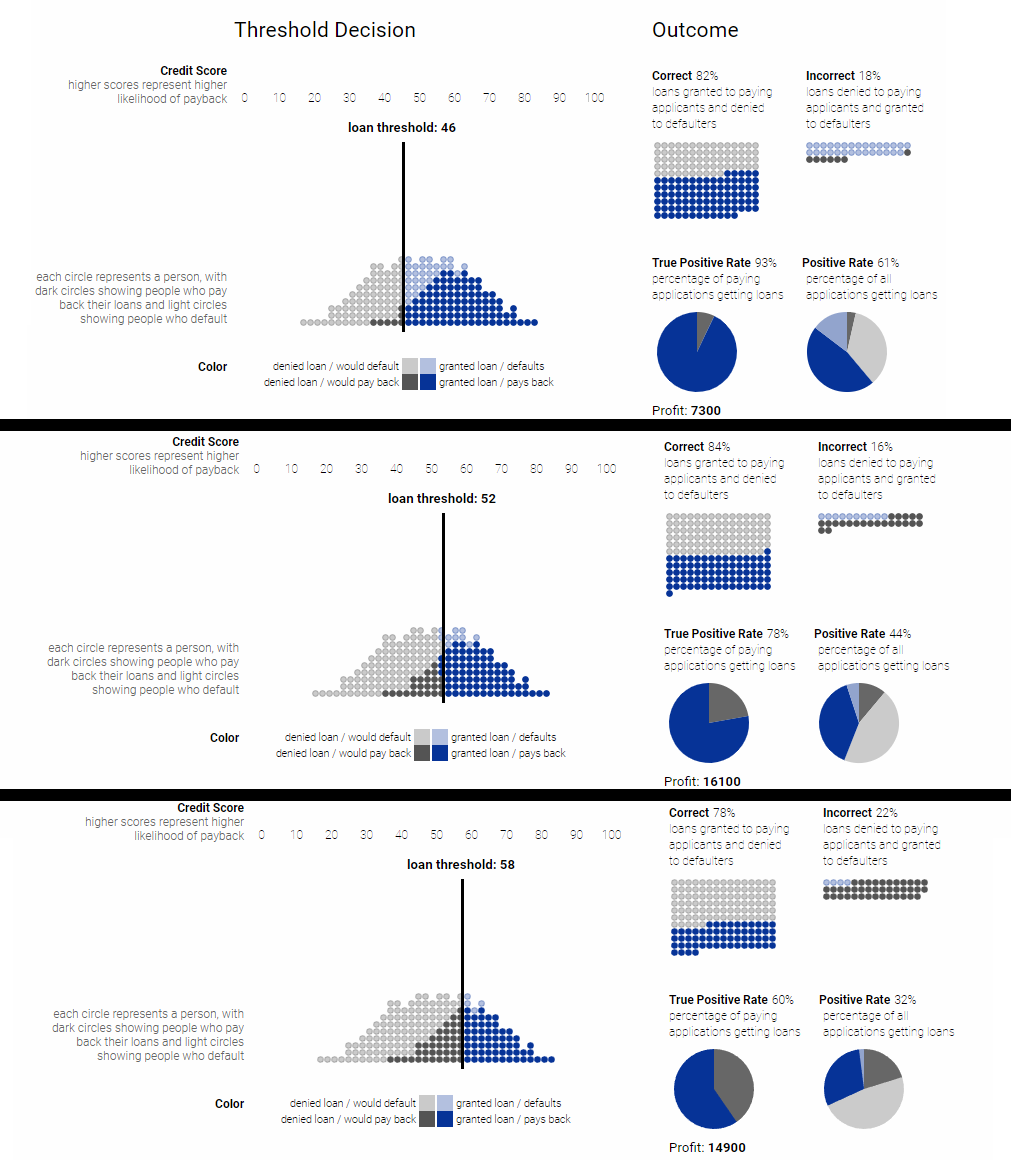
\includegraphics[scale=0.4]{loanML}
\begin{description}
\item Observe tradeoff: 
\begin{itemize}
\item Too low threshold: bank gives loans to many people who default
\item Too high: many people who deserve a loan won't get one
\end{itemize}
\end{description}
\begin{itemize}
\item Different thresholds for different goals (maximize profit, maximize number of correct decisions, ...)
\item Interesting: Threshold of 52 \(\rightarrow\) Correct: 84\%, profit: 16100 \textbf{but} Threshold of 54 \(\rightarrow\) Correct: 83\%, profit: 16600
\end{itemize}
\subsection{Classification and Discrimination}
The definition of ``the correct'' decision depends on the context and is complicated. Consider:
\begin{itemize}
\item Two groups of people, equally likely to pay off loans (overall)
\item Different distribution
\item Depending on the goal (e.g. max profit) the two groups will be held to different standards:
\end{itemize}
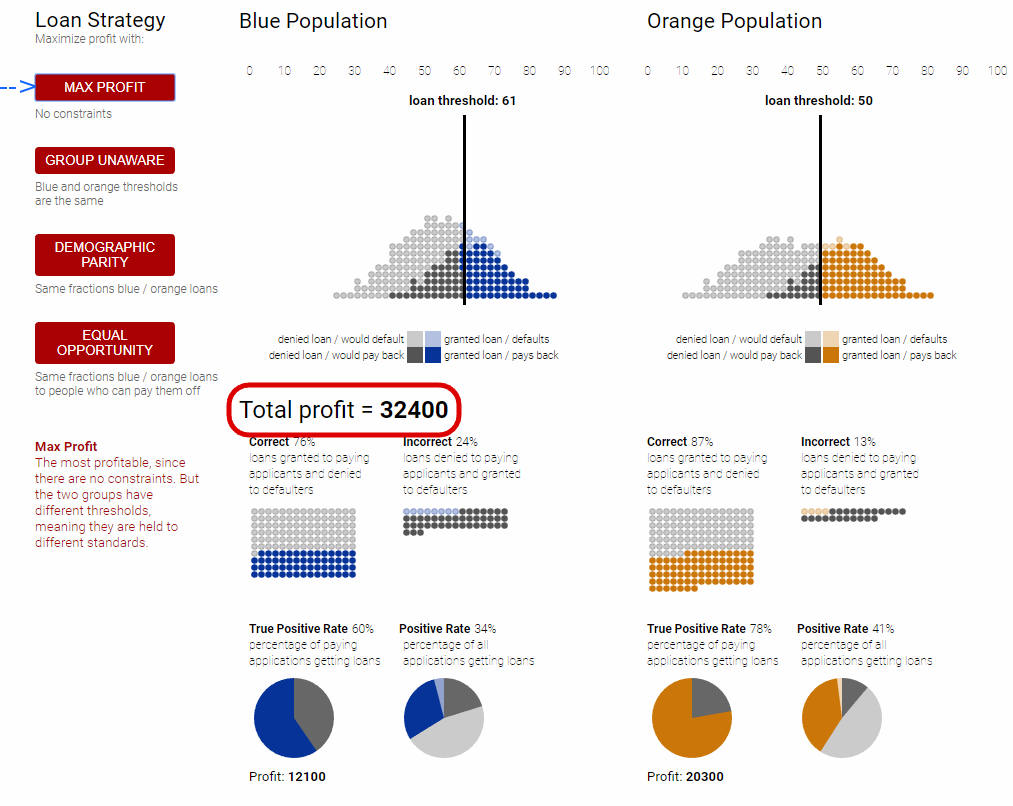
\includegraphics[scale=0.4]{loanML2}
\begin{description}
\item Other strategies:
\end{description}
\begin{itemize}
\item Group-unaware
\begin{itemize}
\item Hold both groups to same standards 
\item Problem: might be unfair to ignore real differences
\end{itemize}
\item Demographic parity 
\begin{itemize}
\item Thresholds yield same fraction of loans to each group (positive rates are equal)
\item Problem: only looks at loans given, not loans paid back \(\rightarrow\) fewer qualified blue people are being given loans than in the orange group
\end{itemize}
\item Equal opportunity (paper by Hardt, Price, Srebro)
\begin{itemize}
\item Of the oeople who can pay back a loan, the same fraction in each group should actually be granted one
\end{itemize}
\end{itemize}
\subsection{Improving machine learning systems}
\begin{itemize}
\item \textit{Key result of the paper:} Given any scoring system it's possible to find thresholds that meet any of these criteria \(\rightarrow\) always possible to attack discrimination
\item Attacking discrimination in ML will require a careful, multidisciplinary approach
\end{itemize}
\end{document}